\chapter{DESARROLLO DEL SISTEMA DE DETECCIÓN}

En este capítulo se describe cómo el sistema de detección de incendios es desarrollado mediante el uso de técnicas de Visión por Computador y Aprendizaje Automático.

Las primeras secciones definen el contexto del ambiente de desarrollo, el diseño mediante el cual el sistema es desarrollado donde se presenta una visión completa del funcionamiento del mismo. Después se aplican los métodos elegidos para el desarrollo de cada uno de los procesos principales que contempla el sistema de detección de incendios.

\section{Contexto del ambiente de desarrollo}

El objetivo de este proyecto de grado es la creación de un sistema de detección visual, por tanto, esta basado sólo en la captura de imagen de una cámara ordinaria. Las razones para esta elección es que, el uso de una cámara ordinaria permite realizar pruebas de manera más fácil y rápida, ya que no es necesario el uso de hardware especial para ejecutarse y el conjunto de datos recolectados durante el desarrollo están disponibles en linea.

Además las cámaras fotográficas normales son más baratas que cámaras térmicas, esto significa que el sistema puede ser implantado a diferentes sistemas a un precio mucho mas accesible.

El sistema fue desarrollado en una computadora personal que tiene las siguientes características:
\begin{itemize}
\item Procesador Cuádruple núcleo Intel® Core™ i3-3217U CPU @ 1.80GHz.
\item 3,8 GiB de memoria ram.
\item Sistema Operativo elementary OS 0.3.2 Freya (64-bit)
\end{itemize}

Todo el código producido en este proyecto de grado ha sido escrito en Python, que es un lenguaje de programación interpretado que esta enfatizado en la simplicidad y legibilidad de código, que se potencia con el apoyo de poderosas librerías científicas tales como NumPy, SciPy, OpenCV, etc.

\section{Alcance del sistema de detección}

El sistema desarrollado para este proyecto de grado debe ser considerado como una prueba de concepto en lugar de una solución final. Se ha tomado en cuenta a lo largo de todo el proyecto, soluciones parciales y/o totales aplicadas en diferentes investigaciones. Entonces el tiempo de procesamiento es tal vez la mayor restricción impuesta en el sistema ya que idealmente el procesamiento debe suceder en tiempo real.

En base al análisis realizado en el capítulo anterior, el sistema esta restringido al procesamiento de imágenes correspondientes a áreas forestales y no así a situaciones suscitadas en otras áreas.

Además, se evidencia que un sistema de detección de incendios totalmente autónomo no va a funcionar de forma aislada, sino que sera parte de un sistema mas grande posiblemente bastante complejo que estará bajo supervisión humana. Entonces, el trabajo realizado se ha centrado en la aplicación de software del sistema de detección de incendios en áreas forestales que sólo utiliza la entrada de una cámara ordinaria, software o hardware adicional que corresponda a un sistema mas completo esta más allá del alcance de este proyecto de grado.

\section{Diseño del sistema de detección}

Para el sistema de detección diseñado en este proyecto de grado se realizan dos detecciones: un detector de fuego basado en el descriptor HOG y un detector de humo basado en LBP. Ambos realizan la detección mediante el clasificador SVM. Entonces cada una de las detecciones esta basado en el diseño presentado en esta sección.

\subsection{Diagrama de procesos}

Para cada una de las detecciones, se genera un modelo clasificador basado en SVM, este sera utilizado recién en el sistema de detección donde sera aplicado a una imagen completa.

\subsubsection{Generación del modelo clasificador}

Como se vio en el capitulo anterior, para generar un modelo clasificador se parte de un conjunto de ejemplos con los cuales se realiza el entrenamiento y se hallan los vectores de soporte que permiten realizar una clasificación.

Entonces, dado un conjunto de imágenes se realiza un proceso manual de anotación para obtener muestras positivas y negativas. Del conjunto de imágenes positivas y negativas, aleatoriamente son asignados en conjuntos de entrenamiento, evaluación y validación.

\begin{figure}[H]
\centering
{\includegraphics[width=1\textwidth , frame]{imagenes/anotacion.png}}
%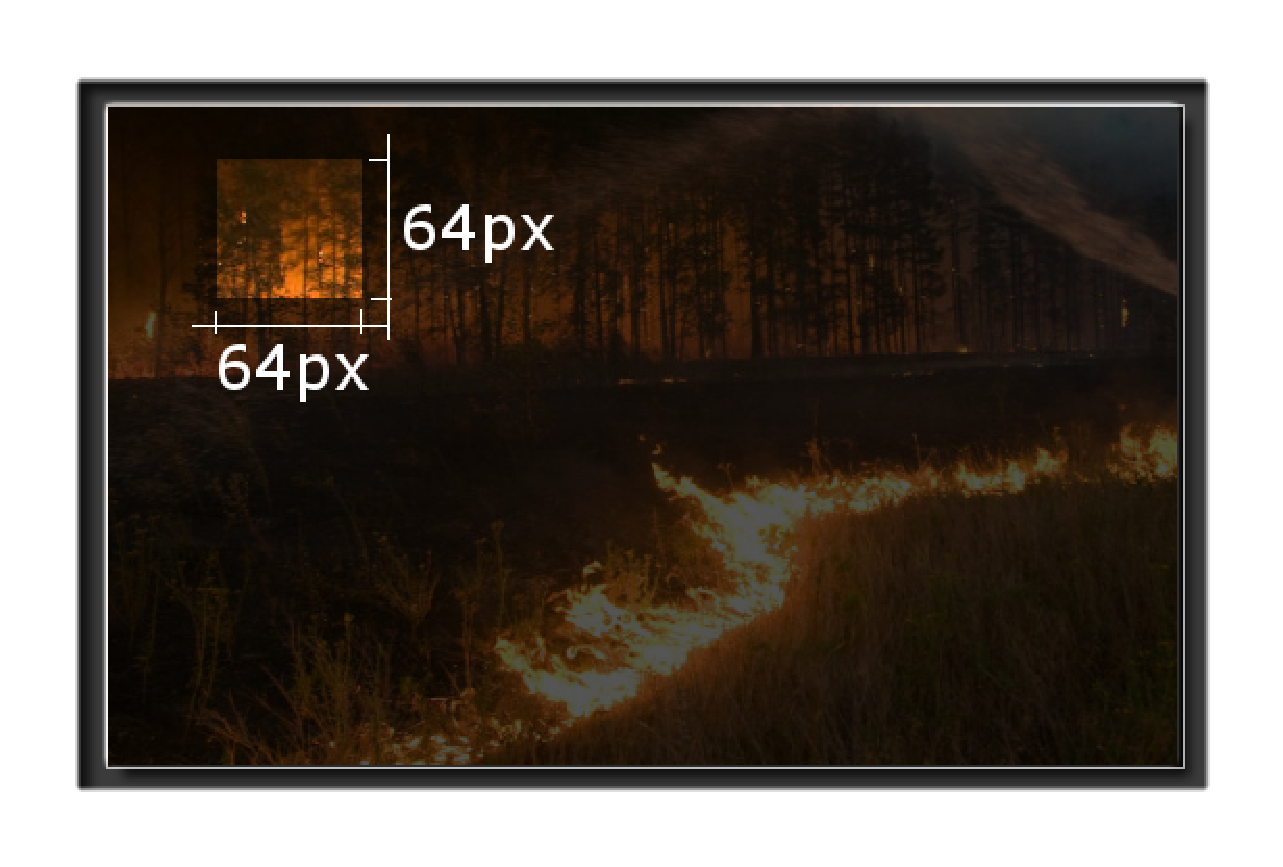
\includegraphics[width=0.5\textwidth , frame]{./imagenes/tratamiento/recorte}
\caption{Sección de la imagen que sera recortada.}
\label{fig:sectorRecorte}
\end{figure}

Luego, para cada imagen del conjunto de entrenamiento, se obtiene su descriptor correspondiente con la etiqueta que le corresponde (si es una muestra positiva o negativa) para generar el modelo clasificador y luego hacer las pruebas sobre las mismas imágenes de entrenamiento. En caso de que las pruebas no satisfagan se realiza un refinamiento de muestras de entrenamiento mediante Bootstraping y Aprendizaje Activo hasta que las pruebas satisfagan en los conjuntos de entrenamiento y evaluación.

\begin{figure}[H]
\centering
{\includegraphics[width=1\textwidth , frame]{imagenes/generacionmodelo.png}}
%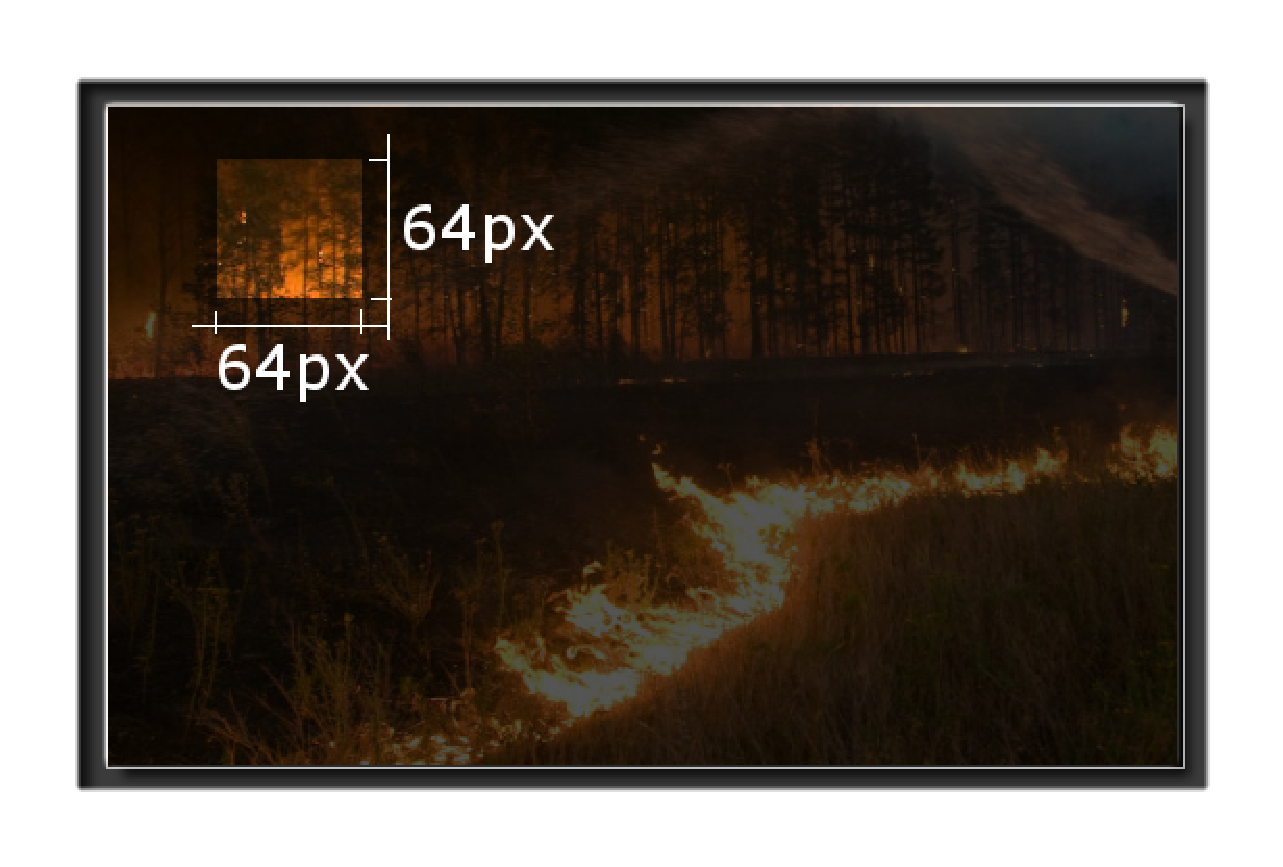
\includegraphics[width=0.5\textwidth , frame]{./imagenes/tratamiento/recorte}
\caption{Sección de la imagen que sera recortada.}
\label{fig:sectorRecorte}
\end{figure}

El modelo entrenado que satisfaga los conjuntos de entrenamiento y evaluación es el modelo que se utilizara para la clasificación en el sistema de detección, realizar la clasificación sobre el conjunto de validación permite evaluar el rendimiento del clasificador, se puede ver mas detalles de esto en el capitulo 4.

\subsubsection{Sistema de detección}

El sistema de detección se aplica sobre una imagen de entrada obtenida con una cámara ordinaria, donde el primer proceso es establecer las regiones de interés dentro de la imagen, entonces se definen los lugares donde podría existir presencia de humo o fuego dentro de la imagen con el uso de técnicas de Visión por Computador relacionados al descriptor de color.

\begin{figure}[H]
\centering
{\includegraphics[width=1\textwidth , frame]{imagenes/sistema.png}}
%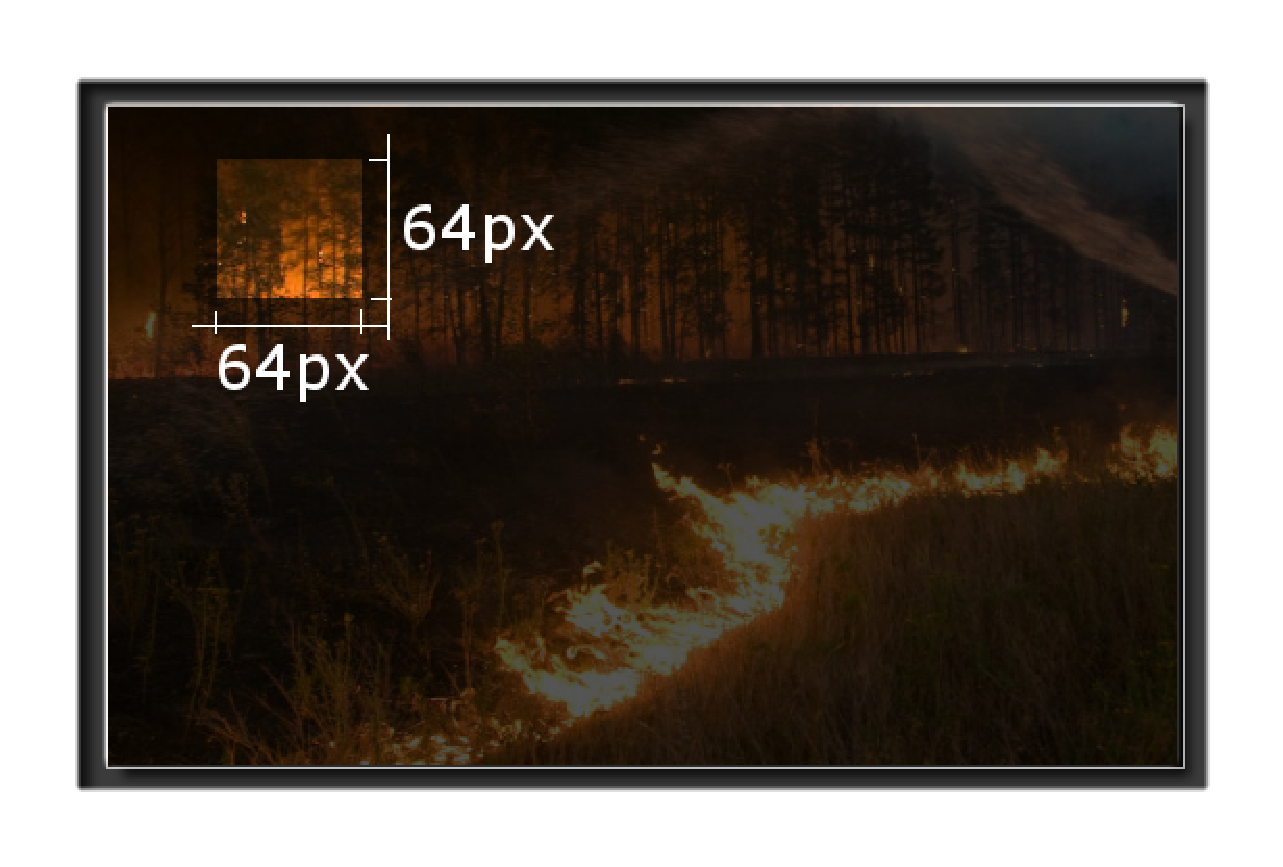
\includegraphics[width=0.5\textwidth , frame]{./imagenes/tratamiento/recorte}
\caption{Sección de la imagen que sera recortada.}
\label{fig:sectorRecorte}
\end{figure}

Entonces en base a estas regiones se generan candidatos que serán evaluados por el modelo clasificador. Por cada candidato se obtiene su descriptor y se evalúa con el modelo entrenado para obtener una resultado.

Debido a que un candidato que haya dado positivo puede solapar a otro candidato en cierto porcentaje dentro de la imagen se realiza una refinación de los resultados sobre la imagen, para que estos sean tomados en cuenta como un solo resultado. Después de este proceso se obtiene la imagen resultante con recuadros en las regiones que se hayan detectado fuego o humo.

\subsection{Rol de actividades}

\noindent Este es el rol de actividades.

\begin{table}[h!]
\begin{center}
\begin{tabular}{|c|p{8 cm}|c|}
\hline 
\textbf{\#} & \textbf{ Hito} & \textbf{Fecha estimada de entrega} \\ 
\hline \hline
1. & Contexto del ambiente de desarrollo & 25 de Mayo \\ 
\hline 
2. & Diseño del sistema & 25 de Mayo \\ 
\hline 
3. & Generación del modelo clasificador & 16 de Junio \\ 
\hline 
4. & Evaluación del modelo clasificador & 16 de Junio \\ 
\hline 
4. & Establecimiento de las regiones de interés & 7 de Julio \\ 
\hline 
5. & Generación del candidatos & 7 de Julio \\ 
\hline 
6. & Clasificación de candidatos & 7 de Julio \\ 
\hline 
7. & Refinación de la clasificación & 28 de Julio \\ 
\hline 
7. & Evaluación del sistema de detección & 28 de Julio \\ 
\hline 
9. & Tabulación de resultados & 11 de Agosto \\ 
\hline 
8. & Entrega preliminar & 11 de Agosto \\ 
\hline 
10. & Entrega final & 18 de Agosto \\ 
\hline 
\end{tabular} 
\caption{Rol de actividades.}
\end{center}
\end{table}

\section{Generación del modelo}

\noindent Esta sección describe el proceso seguido para la generación de los modelos clasificadores detectores de humo y fuego.

\noindent Un modelo entrenado mediante Aprendizaje Supervisado, es capaz de deducir un resultado a partir de datos de entrenamiento. Entonces elegimos un conjunto de muestras etiquetadas con sus respectivas clases, un porcentaje de estas muestras serán elegidas para el entrenamiento, evaluación y validación del modelo clasificador.

\subsection{Selección de imágenes}

\noindent El proceso de anotación se realizara sobre imágenes de incendios en áreas forestales recolectadas de Internet.

\subsubsection{Anotación}
\noindent Algo que caracteriza a un modelo entrado mediante Aprendizaje Supervisado es que solo pueden trabajar con conjuntos de entrenamiento que generen vectores de tamaño fijo. Con el objetivo de cumplir esto es necesario establecer un tamaño fijo para el conjunto de imágenes de entrenamiento. Entonces imágenes que hayan sido seleccionadas que no cumplan con el tamaño elegido, serán procesadas para que cumplan con este requisito.

\noindent El fuego y humo no tienen una relación natural en su altura y anchura, es por este motivo que el tamaño canónico establecido para la generación de candidatos serán cuadrados perfectos.

\subsubsection{Conjunto entrenamiento, evaluación y validación}

\noindent De todo el conjunto de imágenes positivas y negativas generadas mediante la anotación, estos serán divididos aleatoriamente en conjuntos que serán utilizados para el entrenamiento, evaluación y validación del modelo clasificador, mediante la siguiente relación:

\begin{itemize}
\item El 80\% del del conjunto generado pasan al conjunto de entrenamiento.
\item El 10\% del del conjunto generado pasan al conjunto de evaluación.
\item El 10\% del del conjunto generado pasan al conjunto de validación.
\end{itemize}

\noindent Los conjunto de entrenamiento y evaluación, son utilizados para la generación de un modelo que se acerque a resultados óptimos durante la clasificación.

\begin{figure}[H]
\centering
{\includegraphics[width=1\textwidth , frame]{imagenes/1conjuntos.png}}
%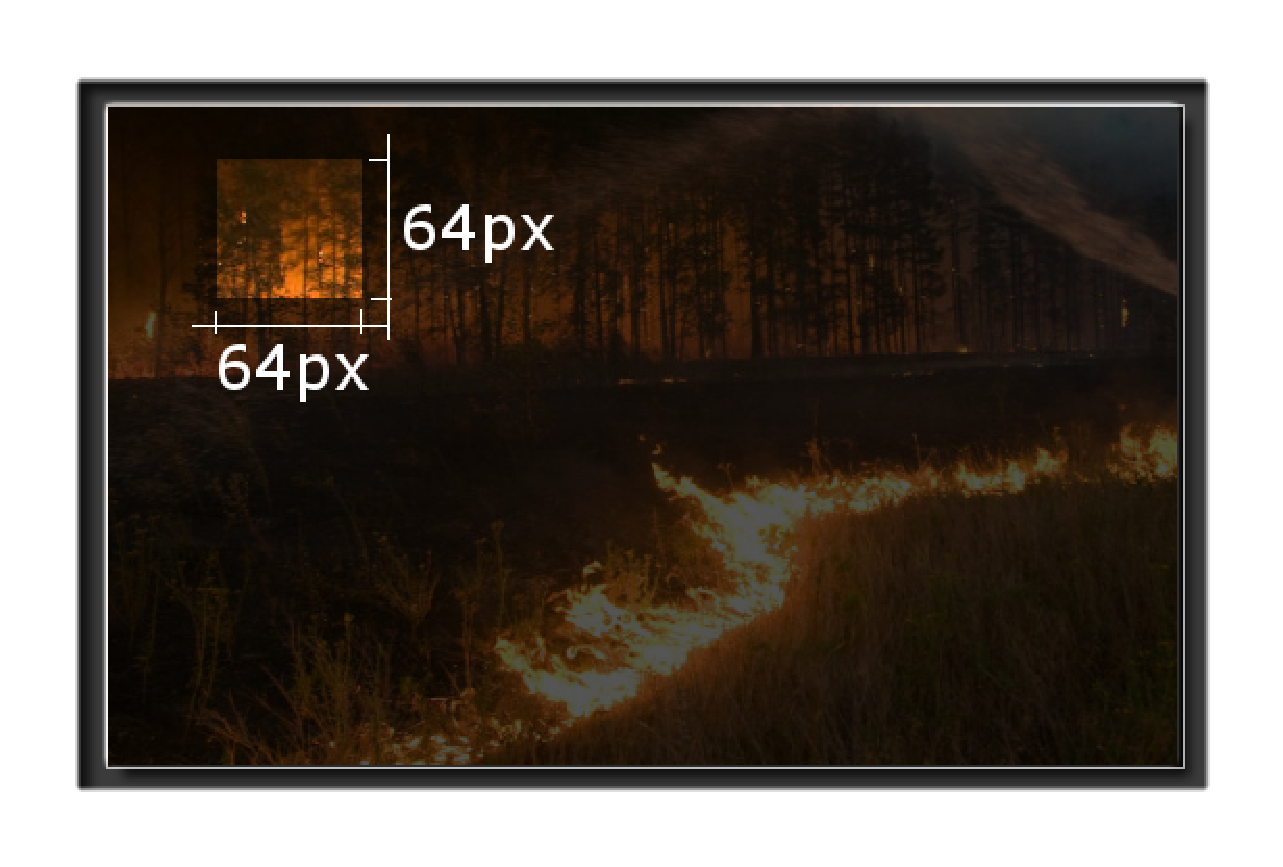
\includegraphics[width=0.5\textwidth , frame]{./imagenes/tratamiento/recorte}
\caption{Sección de la imagen que sera recortada.}
\label{fig:sectorRecorte}
\end{figure}

\noindent El conjunto de validación es un conjunto aislado, donde ninguno de los elementos estuvo involucrado con el entrenamiento del modelo. Este conjunto permite establecer la calidad del modelo clasificador.

\subsection{Entrenamiento}

\noindent Primero, de cada elemento del conjunto de entrenamiento se obtienen sus descriptores y se le añade la etiqueta a la cual corresponde (si son muestras positivas o negativas). Estos son almacenados en una matriz donde cada fila es el descriptor de una muestra mas su correspondiente etiqueta y el numero de columnas es la cantidad de muestras de entrenamiento.

\begin{figure}[H]
\centering
{\includegraphics[width=1\textwidth , frame]{imagenes/1matriz.png}}
%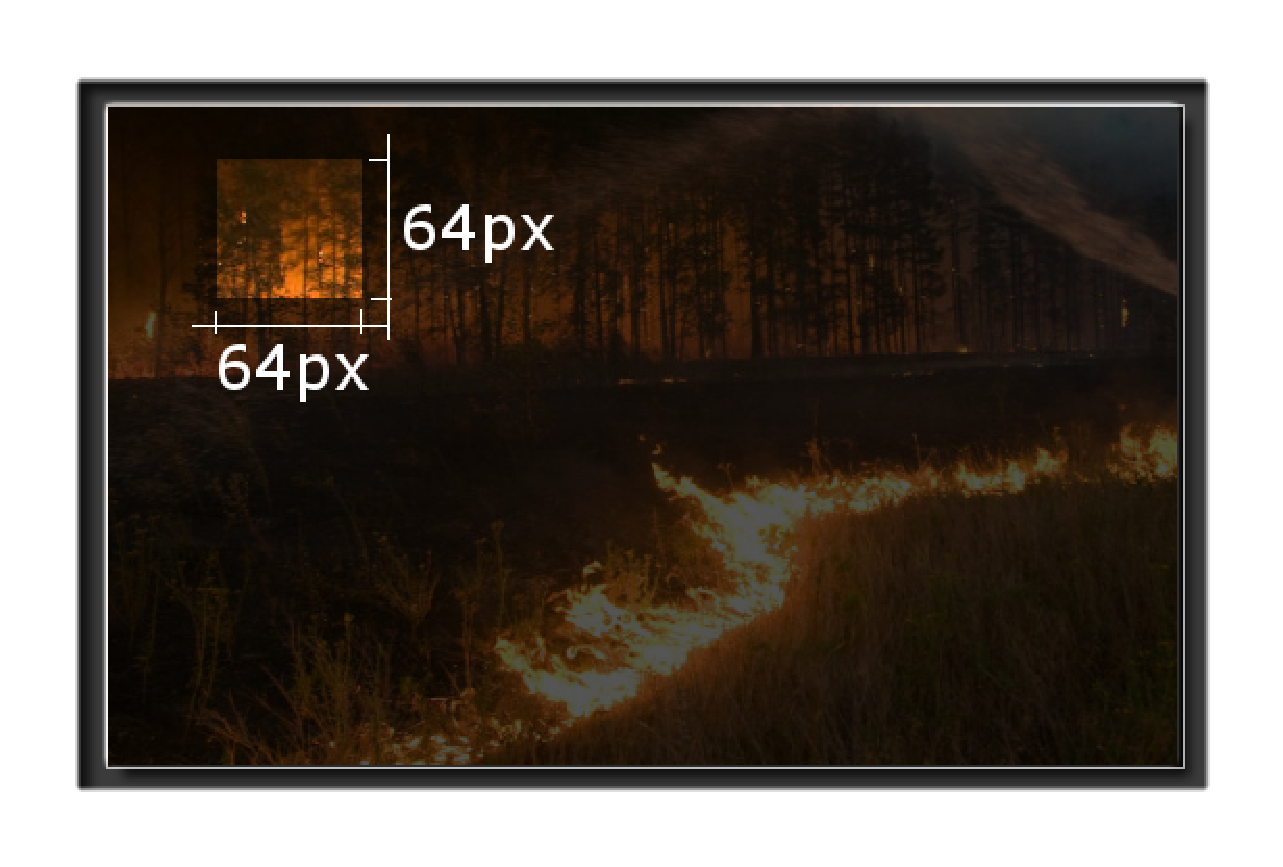
\includegraphics[width=0.5\textwidth , frame]{./imagenes/tratamiento/recorte}
\caption{Sección de la imagen que sera recortada.}
\label{fig:sectorRecorte}
\end{figure}

\noindent Esta matriz pasa por el entrenamiento SVM, y genera un modelo entrenado que contiene los vectores de soporte que representan el limite de detección para decir si una muestra es positiva o negativa.

\subsection{Refinación}

\noindent Aunque el entrenamiento es generado en un solo paso, nada garantiza la calidad de predicción del mismo, es por este motivo que en un proceso iterativo se refina el entrenamiento hasta que cumpla con los conjuntos de entrenamiento y validación.

\begin{figure}[H]
\centering
{\includegraphics[width=1\textwidth , frame]{imagenes/1refinacion.png}}
%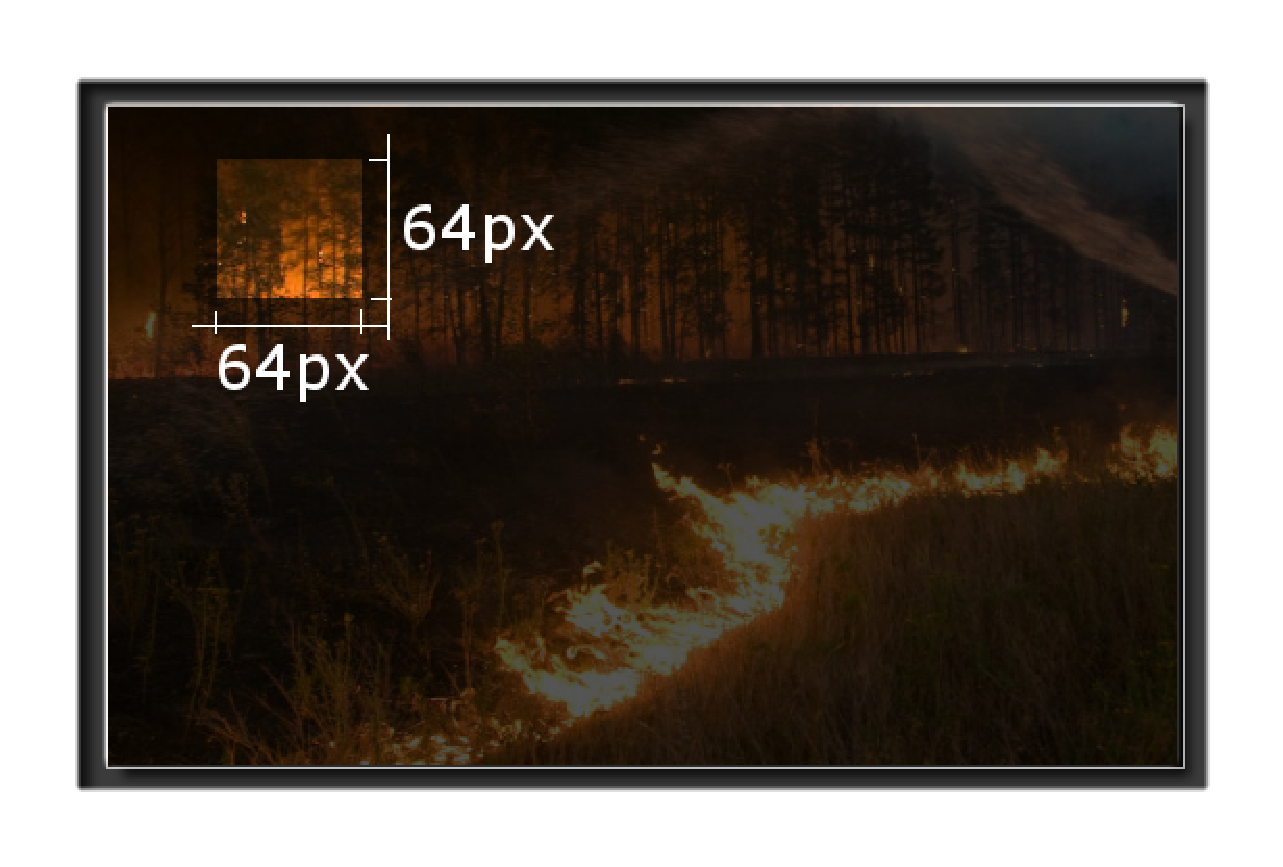
\includegraphics[width=0.5\textwidth , frame]{./imagenes/tratamiento/recorte}
\caption{Sección de la imagen que sera recortada.}
\label{fig:sectorRecorte}
\end{figure}

\noindent En el plano donde se representan los vectores de soporte hallados por la Maquina de Soporte Vectorial, se puede distinguir ejemplos que se encuentran mas cercanos a los vectores de soporte. Entonces el modelo asume que estos puntos son los mas difíciles de predecir, mientras que un punto que esta alejado de los vectores de soporte, su predicción esta polarizada a positivo o negativo.

\noindent Las técnicas de refinación presentadas a continuación pretenden ayudan a refinar los vectores de soporte generados mediante el entrenamiento iterativo, para que la predicción sea mas eficiente.

\subsubsection{Bootstraping}

\noindent Boostraping pone a prueba el modelo clasificador con las muestras negativos del conjunto de entrenamiento en busca de detección de falsos positivos. Entonces todos los resultados que estén próximos a los vectores de soporte (ya sean falsos negativos o falsos positivos) son los negativos difíciles y pasan a ser el nuevo conjunto de negativos para el próximo entrenamiento.

\begin{figure}[H]
\centering
{\includegraphics[width=1\textwidth , frame]{imagenes/1bootstraping.png}}
%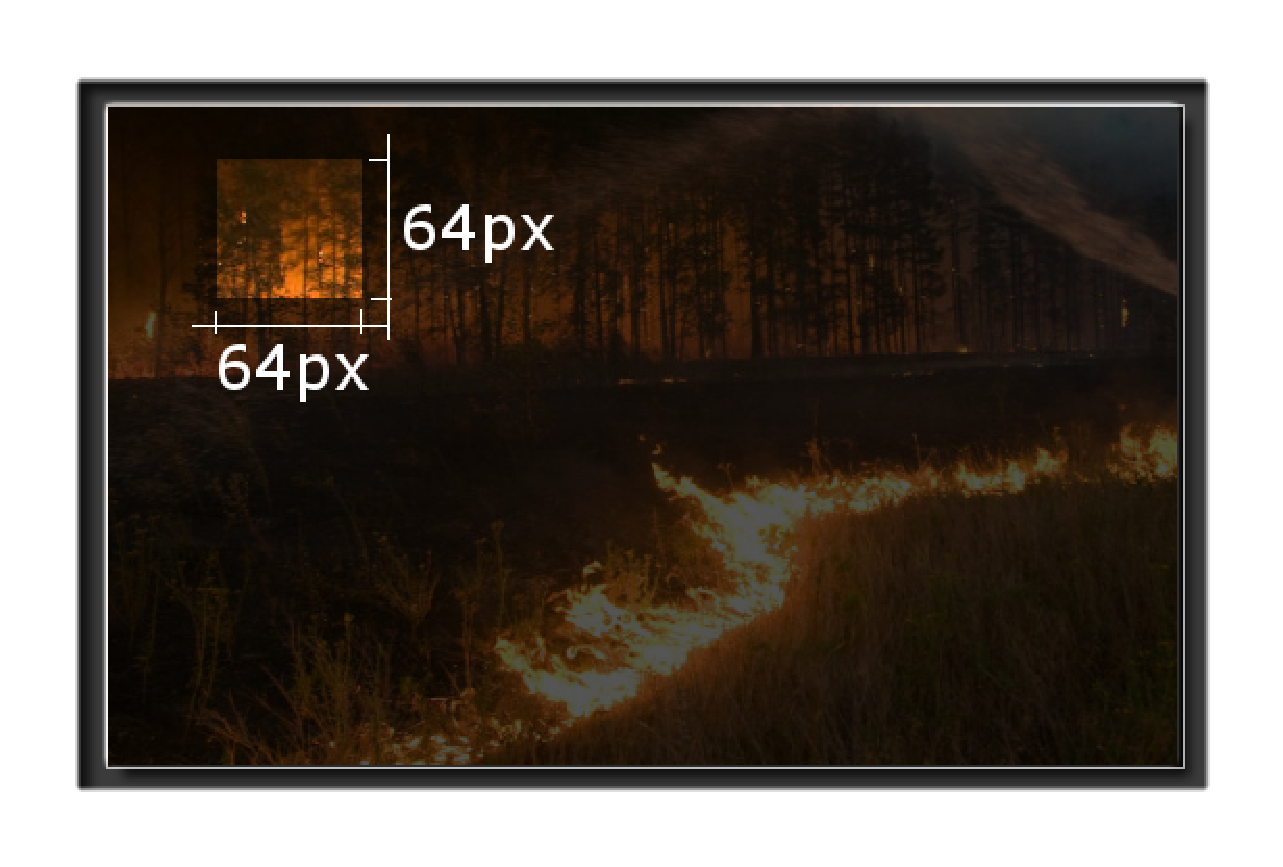
\includegraphics[width=0.5\textwidth , frame]{./imagenes/tratamiento/recorte}
\caption{Sección de la imagen que sera recortada.}
\label{fig:sectorRecorte}
\end{figure}

\noindent De esta manera se evita el peso que generan en el modelo aquellos negativos fáciles (aquellos que están lejos, de los vectores de soporte) y se obtiene un modelo que ajusta mas a la predicción.

\noindent En cuanto el modelo ya no detecte falsos positivos, en las muestras negativas del conjunto de entrenamiento, se pasa a realizar el mismo procedimiento sobre el conjunto de evaluación, añadiendo los falsos positivos que se vayan detectando al conjunto de negativos.

\subsubsection{Aprendizaje activo}

\noindent En el Aprendizaje Activo se ponen a prueba las muestras positivas y negativas del conjunto de entrenamiento, de los resultados obtenidos.

\noindent De los resultados de las muestras positivas, aquellas que están próximas a los vectores de soporte son los positivos difíciles y estas pasaran a ser las muestras en el conjunto de positivos para el próximo entrenamiento.

\begin{figure}[H]
\centering
{\includegraphics[width=1\textwidth , frame]{imagenes/1aprendizajeactivo.png}}
%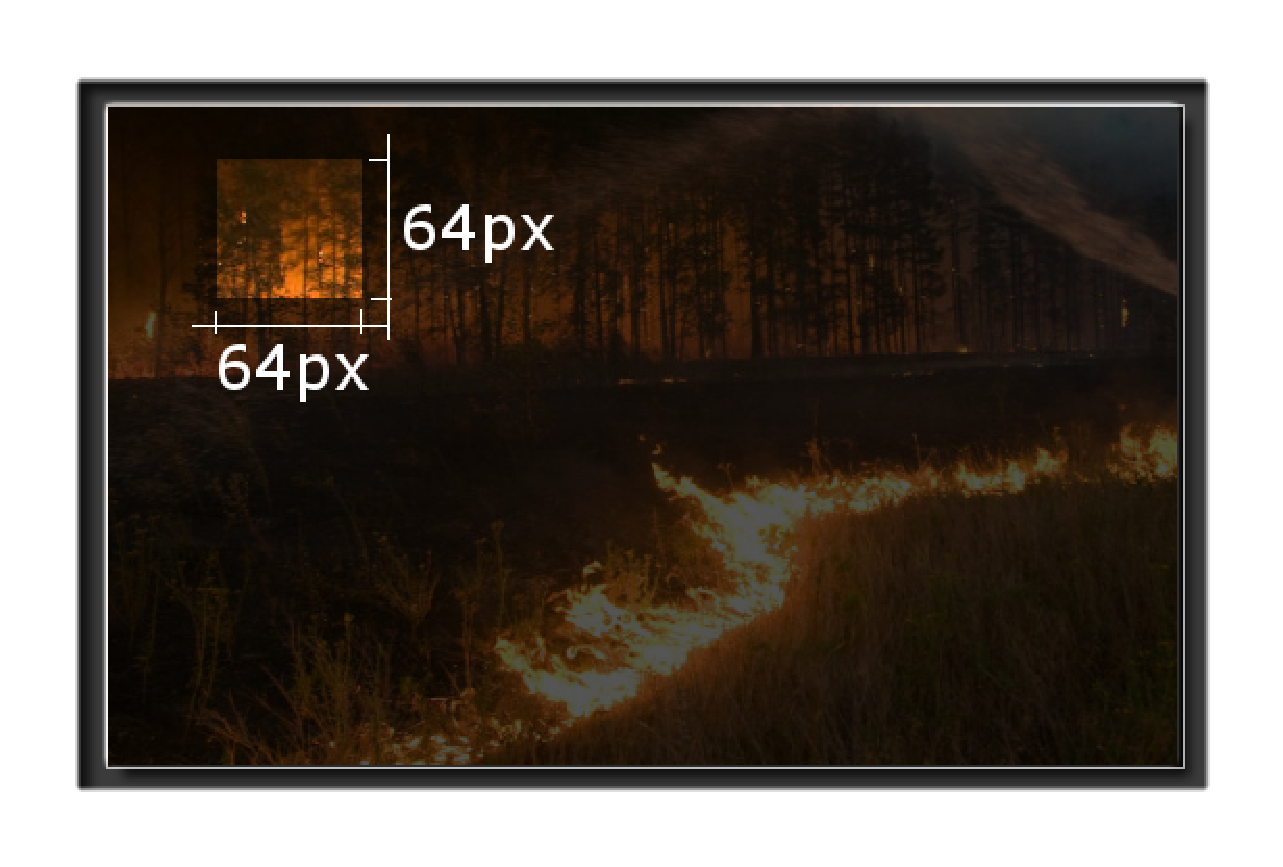
\includegraphics[width=0.5\textwidth , frame]{./imagenes/tratamiento/recorte}
\caption{Sección de la imagen que sera recortada.}
\label{fig:sectorRecorte}
\end{figure}

\noindent Las pruebas realizadas sobre las muestras negativas, permiten verificar que los nuevos modelos generados no generan falsos positivos ocasionando que el modelo clasificador no haga la predicción de manera correcta. En caso de que se vayan encontrando falsos positivos estos deben ser añadidos al conjunto de negativos para el próximo entrenamiento.

\noindent Entonces, el entrenamiento refinado que satisface los conjuntos de entrenamiento y evaluación es el entrenamiento final que sera utilizado en el sistema de detección. En el capitulo 4 se procede a evaluar el rendimiento del modelo clasificador con el conjunto de validación.

\section{Implementación del sistema de detección}

\noindent En esta sección se detalla la implementación del sistema de detección de incendios. El sistema realiza la detección sobre una imagen completa, se seleccionan las regiones que nos interesan analizar con el modelo clasificador. De estas regiones se generan candidatos que el modelo clasificador pueda predecir si es una región que contiene fuego, humo o ninguno de los 2.

\subsection{Establecer las regiones de interés}

\noindent Este proceso permite discriminar regiones que no tengan posibilidad de ser fuego o humo. De esta manera mediante el descriptor del color de pixel se obtiene regiones que tengan al menos una ligera posibilidad de ser fuego o humo.

\subsection{Generación de candidatos}

\noindent En base a las regiones de interés obtenidas en el proceso anterior, se generan candidatos que son muestras de estas regiones del tamaño correspondiente para poder realizar la detección mediante el modelo clasificador. Las técnicas utilizadas para poder realizar esta detección son la de ventana deslizante y incremento piramidal.

\subsubsection{Ventana deslizante}

\noindent Dado el tamaño canónico elegido para la detección de humo y fuego, se generan candidatos por toda la superficie de las regiones de interés.

\noindent Entonces se toma un candidato del extremo superior izquierdo de la región de interés, se define el salto como el recorrido que queremos darle para la generación del siguiente candidato. Este proceso se repite por toda la superficie de cada una de las regiones de interés, obteniendo como resultado una colección de candidatos.

\subsubsection{Pirámide}

\noindent Con el paso anterior se generan todos los candidatos en las regiones de interés, pero solo de tamaño canónico. Entonces si tenemos la presencia de humo o fuego mas cerca, se generaron candidatos que corresponden a la mitad de una imagen de humo o fuego.

\noindent Para obtener candidatos que correspondan a diferentes tamaños de la región de interés, se hace un cambio de dimensión a la imagen original (mas pequeño), mantenemos el tamaño de generación de candidatos y se repite el proceso de ventana deslizante sobre la imagen redimensionada. Este proceso se repite hasta que el tamaño de la ventana de generación de candidatos sea mayor a cualquier región de interés del cual se generan candidatos.

\subsection{Extracción de características}

\noindent En este punto, se tiene una colección de candidatos de fuego y/o humo que deben ser sometidos a una predicción por sus respectivos modelos de clasificación.

\noindent Entonces de cada uno de estos candidatos se obtiene su respectivo descriptor. El descriptor de los candidatos de fuego se obtiene mediante el algoritmo HOG y los de humo mediante el algoritmo LBP.

\noindent La colección de candidatos pasa a ser una colección de descriptores y están listos para ser sometidos a una clasificación.

\subsection{Clasificación de candidatos}

\noindent El siguiente paso, es la clasificación de la colección de descriptores generados a partir de las regiones de interés. Para ello se carga los modelos clasificadores de fuego y humo entrenados en la sección anterior y cada elemento de la colección de descriptores debe someterse a la predicción de su correspondiente modelo.

\noindent En base a los resultados obtenidos de cada clasificador, se tiene las regiones donde se detecto la presencia de humo o fuego.

\subsection{Refinación de la clasificación}

\noindent La clasificación obtenida sobre la imagen en el proceso anterior necesita una refinación por que puede existir cierto porcentaje de solapamiento en las detecciones obtenidas. Entonces definimos un porcentaje mínimo de solapamiento que debe existir para que 2 detecciones sean tomadas como una, recorremos la colección de detecciones buscando este solapamiento para obtener una clasificación refinada.

\section{Resumen del capitulo}
